\documentclass[aspectratio=169]{beamer}

\usetheme{metropolis}
\usepackage{appendixnumberbeamer}

\usepackage{booktabs}
\usepackage[scale=2]{ccicons}

\usepackage{pgfplots}

\usepackage{xspace}
\newcommand{\themename}{\textbf{\textsc{metropolis}}\xspace}

\usepackage[utf8]{inputenc}
\usepackage[T1]{fontenc}

\usepackage{listings}
\usepackage{xcolor, colortbl}
\usepackage{multicol}
\usepackage{chronology}

\usepackage[]{algorithm2e}
\usepackage{hyperref}

\definecolor{done}{rgb}{0.36, 0.72, 0.36}
\definecolor{doing}{rgb}{1.0, 0.8, 0.0}
\definecolor{scheduled}{rgb}{0.25, 0.54, 0.79}


\newcommand{\done}{\cellcolor{done}}
\newcommand{\scheduled}{\cellcolor{scheduled}}
\newcommand{\doing}{\cellcolor{doing}}

\bibliographystyle{unsrt}

\lstdefinestyle{sharpc}{language=[Sharp]C, frame=lr, rulecolor=\color{blue!80!black}}

\title{Domain-Driven Design: Parte I}
\date{}
\author{Johnathan Fercher}
%\institute{Braspag}
\titlegraphic{\hfill
\includegraphics[height=1.1cm]{imgs/logo.png}}

\newcommand{\ubiquitouslanguagesample}{Ex: Uma \textbf{pessoa} possui \textbf{cartões de créditos}. \textbf{Cartões de créditos} podem ser utilizados em \textbf{transações}. Quando uma \textbf{transação} é realizada com um \textbf{cartão de crédito} sem permissão, a mesma se caracteriza como \textbf{fraude}. Uma \textbf{fraude} pode acarretar em um \textbf{chargeback}. Quando um \textbf{chargeback} ocorre, o \textbf{cartão de crédito} vinculado aquela \textbf{transação} é cancelado.}

\begin{document}
\maketitle

\begin{frame}{Sumário}
  \setbeamertemplate{section in toc}[sections numbered]
  \tableofcontents[hideallsubsections]
\end{frame}

\section{Introdução}
\begin{frame}{DDD não é uma biblioteca/framework}	
	\begin{itemize}	
		\item C\#: Install-Package DomainDrivenDesign
		\item Python: pip install domain\_driven\_design
		\item JavaScript: npm install --save domain\_driven\_design
		\item Rust: ddd = "1.0.1"
		\item C++: 
		\begin{itemize}	
			\item git clone https://github.com/eric-evans/ddd-devcpp
			\item cd ddd-devcpp
			\item mkdir build
			\item cd build
			\item cmake ..
			\item make
			\item sudo make install
		\end{itemize}
	\end{itemize}
\end{frame}

\begin{frame}{O que é DDD?}	
	\begin{itemize}	
		\item O que é um Domínio?
		\item O que é um Modelo?
		\item O que é um Design?
	\end{itemize}
\end{frame}

\begin{frame}{O que é um Domínio?}	
	\begin{itemize}	
		\item Uma esfera de conhecimento;
		\item Uma área de interesse ao qual um programa é criado para lidar;
		\item Regras de negócio;
	\end{itemize}

	\ubiquitouslanguagesample
\end{frame}

\begin{frame}{O que é um Modelo?}
	\begin{itemize}	
		\item Um sistema de abstrações que descreve os aspectos mais importantes de um domínio;
	\end{itemize}
\end{frame}

\begin{frame}{O que é um Modelo?}	
	\begin{multicols}{2}		
		\begin{itemize}	
			\item \textbf{Pessoa}
			\begin{itemize}	
				\item Id;
				\item Nome;
				\item Cartões;
			\end{itemize}
		\end{itemize}
		\begin{itemize}	
			\item \textbf{Cartão}
			\begin{itemize}	
				\item HashNumber;
				\item HashHolderName;
				\item ExpirationDate;
				\item Brand;
				\item IsActive;
			\end{itemize}
		\end{itemize}
		\begin{itemize}	
			\item \textbf{Transação}
			\begin{itemize}	
				\item Id;
				\item Data;
				\item Valor;
				\item Cartão;
				\item Pessoa;
			\end{itemize}
		\end{itemize}
		\begin{itemize}	
			\item \textbf{Chargeback}
			\begin{itemize}	
				\item Id;
				\item Transação;
				\item IsFraud;
			\end{itemize}
		\end{itemize}
	\end{multicols}
\end{frame}

\begin{frame}{O que é um Design?}	
	\begin{itemize}	
		\item Implementação do software;
		\item Aspectos técnicos: performance, reusabilidade, segurança, tolerância a falhas, escalabilidade e etc;
	\end{itemize}
	Vamos armazenar as \textbf{transações} em um \textbf{Redis}. Vamos utilizar um \textbf{facade} que tente obter os valores no \textbf{cache}, caso não ache ele vai no \textbf{banco}. 
\end{frame}

\begin{frame}{O que é DDD?}	
	\begin{itemize}	
		\item Uma abordagem de desenvolvimento de software iterativo para sistemas complexos que busca ligar o design ao modelo.
	\end{itemize}
\end{frame}

\begin{frame}{Por que é importante ligar o design ao modelo?}	
	\begin{itemize}	
		\item Um software útil não pode ser desacoplado da realidade do domínio;
		\item Um domínio pode ser abstraído em um modelo de formas diferentes.
		\item Um modelo pode ser implementado de formas diferentes;
		\item Um modelo construído somente visando as regras de negócio pode ser péssimo de se implementar e manter;
		\item Um design construído somente visando aspectos técnicos pode não resolver o problema do domínio de forma satisfatória.
	\end{itemize}
\end{frame}

\begin{frame}{O que é necessário para realizar essa ligação?}	
	\begin{itemize}	
		\item Os especialistas de domínio devem construir o modelo em conjunto com os desenvolvedores; (Planning)
		\item Mudanças no modelo devem refletir no código e mudanças no código devem refletir no modelo. (Refactoring)
		\item Especialistas de domínio e desenvolvedores devem utilizar a \textbf{linguagem ubíqua}.
	\end{itemize}
\end{frame}

\begin{frame}{O que é necessário para realizar essa ligação?}	
	\begin{itemize}	
		\item É interessante que o software seja construído usando algum \textbf{padrão arquitetural} que isole o domínio e mantenha um baixo acoplamento e uma alta coesão entre camadas. 
		\item O modelo deve ser construído utilizando os \textbf{blocos de construção}.
	\end{itemize}
\end{frame}

\begin{frame}{Ligação de DDD com Desenvolvimento Ágil}	
	\begin{center}
		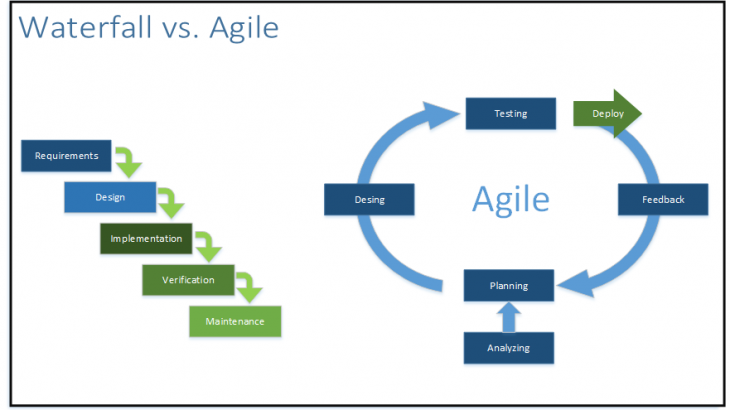
\includegraphics[width=11cm]{imgs/agile-waterfall}
	\end{center}
\end{frame}

\begin{frame}{Devo ou não devo usar DDD?}	
	\begin{multicols}{2}		
		\begin{itemize}	
			\item Usar uma biblioteca de IA para aprender e gerar um artefato;
			\item Escrever o controle embarcado de um robô;
			\item Escrever um \textit{console application} para tratar algo pontual;
			\item Coisas simples; 
		\end{itemize}
		\begin{itemize}	
			\item Construir uma API de OAuth;
			\item Construir um sistema de pagamentos;
			\item Criar um jogo;
			\item Qualquer coisa complexa, onde o domínio precisa ser muito bem compreendido;
		\end{itemize}
	\end{multicols}
\end{frame}

\begin{frame}{O que custa mais caro?}	
	\begin{multicols}{2}		
		\begin{itemize}	
			\item Errar uma abstração de um modelo.
			\begin{itemize}	
				\item Ex: A tabela X deveria ser na verdade duas tabelas. E essas tabelas possuem casos de uso e responsabilidades totalmente diferentes.
			\end{itemize}
		\end{itemize}
		\begin{itemize}	
			\item Errar a implementação de um aspecto de um modelo.
			\begin{itemize}	
				\item Ex: Não contava que teriamos que paralelizar esse processamento, não vai ser possível usar um \textbf{decorator}. Podemos utilizar um \textbf{composite}.
			\end{itemize}
		\end{itemize}
	\end{multicols}
\end{frame}

\section{Linguagem Ubíqua}
\begin{frame}{Linguagem Ubíqua ou Linguagem Onipresente}	
	\begin{itemize}	
		\item Formas de expressar um modelo: diagramas, casos de uso, desenhos e etc;
		\item Tudo isso precisa ser atualizado constantemente;
		\item A fala/escrita é usada de forma constante. Se algo soa errado, provavelmente está errado.
		\item Por que não fazer a fala/escrita nossa representação do modelo?
	\end{itemize}
\end{frame}

\begin{frame}{Linguagem Ubíqua ou Linguagem Onipresente}
	Ex: Um \textbf{cartão de crédito} realiza uma \textbf{transação}. Uma \textbf{transação} pode ser uma \textbf{fraude}.
\end{frame}

\begin{frame}[noframenumbering]{Linguagem Ubíqua ou Linguagem Onipresente}
	Ex: Um \textbf{cartão de crédito} realiza uma \textbf{transação}. Uma \textbf{transação} pode ser uma \textbf{fraude}. Um \textbf{chargeback} é uma \textbf{fraude}.
\end{frame}

\begin{frame}[noframenumbering]{Linguagem Ubíqua ou Linguagem Onipresente}
	Ex: Um \textbf{cartão de crédito} realiza uma \textbf{transação}. Uma \textbf{transação} pode ser uma \textbf{fraude}. Um \textbf{chargeback} pode acarretar em uma \textbf{fraude}.
\end{frame}

\begin{frame}[noframenumbering]{Linguagem Ubíqua ou Linguagem Onipresente}
	Ex: Uma \textbf{pessoa} possui \textbf{cartões de créditos}. \textbf{Cartões de créditos} podem ser utilizados em \textbf{transações}. Uma \textbf{transação} pode ser uma \textbf{fraude}. Um \textbf{chargeback} pode acarretar em uma \textbf{fraude}.
\end{frame}

\begin{frame}[noframenumbering]{Linguagem Ubíqua ou Linguagem Onipresente}
	Ex: Uma \textbf{pessoa} possui \textbf{cartões de créditos}. \textbf{Cartões de créditos} podem ser utilizados em \textbf{transações}. Quando uma \textbf{transação} é realizada com um \textbf{cartão de crédito} sem permissão, a mesma se caracteriza como \textbf{fraude}. Um \textbf{chargeback} pode acarretar em uma \textbf{fraude}.
\end{frame}

\begin{frame}[noframenumbering]{Linguagem Ubíqua ou Linguagem Onipresente}
	\ubiquitouslanguagesample
\end{frame}

\begin{frame}{Linguagem Ubíqua ou Linguagem Onipresente}	
	\begin{center}
		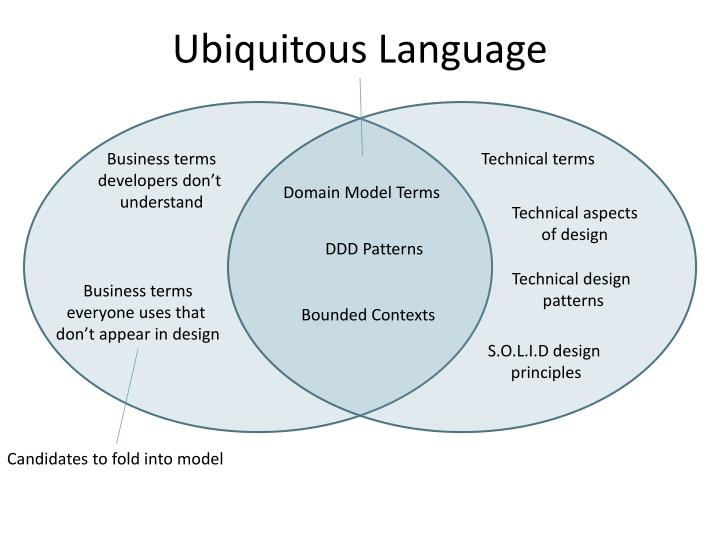
\includegraphics[width=11cm]{imgs/ubiquitous-language}
	\end{center}
\end{frame}


\section{Padrões Arquiteturais}
\begin{frame}{O que são padrões arquiteturais?}	
	\begin{itemize}	
		\item Meios utilizados para isolar partes de um sistema de maneira coesa e desacoplada;
		\item São validados em aplicações reais por diferentes arquitetos em diferentes domínios;
	\end{itemize}
\end{frame}

\begin{frame}{O que isso tem a ver com DDD?}	
	\begin{itemize}	
		\item Um software é constituído de coisas além das regras de negócio;
		\item Existem questões como: interface de usuário, autenticação, autorização, cache, banco de dados e etc;
		\item Isolando o domínio, garantimos coesão e desacoplamento relacionado aos outros aspectos do sistema;
		\item Podemos estender esse isolamento para todas as outras partes; 
	\end{itemize}
\end{frame}

\begin{frame}{Arquitetura em Camadas (Clássica)}	
	\begin{center}
		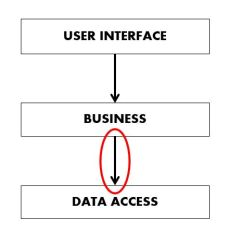
\includegraphics[width=5cm]{imgs/layered-architecture}
	\end{center}
\end{frame}

\begin{frame}{Arquitetura em Camadas (Clássica)}	
	\begin{multicols}{2}		
		\begin{center}
			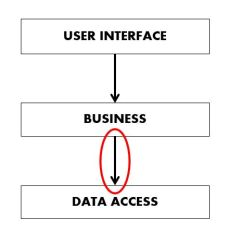
\includegraphics[width=5cm]{imgs/layered-architecture}
		\end{center}
		\begin{itemize}	
			\item \textbf{Business} carrega as regras de negócio e é consequentemente o domínio;
			\item \textbf{User Interface} depende de \textbf{Business} que depende de \textbf{Data Access};
			\item \textbf{Business} pode quebrar caso \textbf{Data Access} mude;
			\item \textbf{Business} deveria ser a camada com menores chances de quebrar, ela não deveria depender de ninguém.
		\end{itemize}
	\end{multicols}
\end{frame}

\begin{frame}{Arquitetura em Camadas (Com foco no Negócio)}			
	\begin{center}
		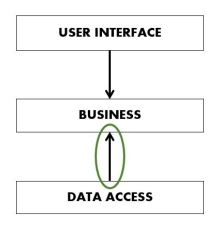
\includegraphics[width=5cm]{imgs/dip-layered-architecture}
	\end{center}
\end{frame}

\begin{frame}{Arquitetura em Camadas (Com foco no Negócio)}	
	\begin{multicols}{2}		
		\begin{center}
			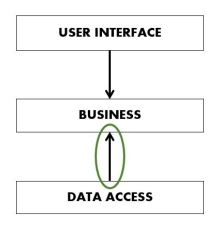
\includegraphics[width=5cm]{imgs/dip-layered-architecture}
		\end{center}
		\begin{itemize}	
			\item Foi aplicado o \textit{Dependency Inversion Principle} de \textbf{Data Access} para \textbf{Business};
			\item \textbf{Business} agora não depende de ninguém e somente quebra com mudanças de negócio;
		\end{itemize}
	\end{multicols}
\end{frame}

\begin{frame}{Arquitetura de Cebola}			
	\begin{center}
		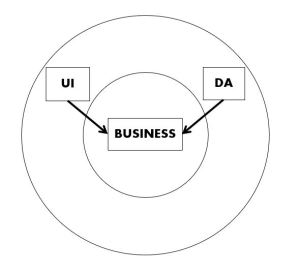
\includegraphics[width=6cm]{imgs/onion-architecture}
	\end{center}
\end{frame}

\begin{frame}{Arquitetura de Cebola}	
	\begin{multicols}{2}		
		\begin{center}
			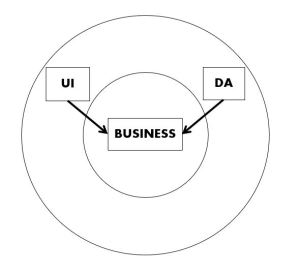
\includegraphics[width=6cm]{imgs/onion-architecture}
		\end{center}
		\begin{itemize}	
			\item Também isola a camada \textbf{Business};
			\item O \textit{Release Equivalence Principle} é violado, pois  alterações na camada \textbf{UI} afetam a versão de \textbf{DA}, e vice-versa. 
			\item O \textit{Common Closure Principle} é violado, pois a camada muda por razões de \textbf{UI} e \textbf{DA}. 
			\item O \textit{Common Reuse Principle} é violado, pois \textbf{DA} não poderia ser reutilizado sem que dependências de \textbf{UI} sejam levadas juntas, e vice-versa.
		\end{itemize}
	\end{multicols}
\end{frame}

\begin{frame}{Arquitetura Hexagonal}			
	\begin{center}
		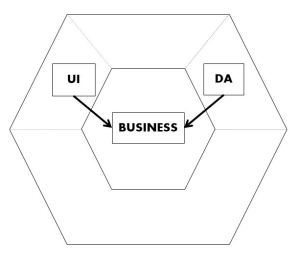
\includegraphics[width=6cm]{imgs/hexagonal}
	\end{center}
\end{frame}

\begin{frame}{Arquitetura Hexagonal}			
	\begin{itemize}	
		\item Também isola a camada \textbf{Business};
		\item O \textit{Release Equivalence Principle} é violado, pois  alterações na camada \textbf{UI} afetam a versão de \textbf{DA}, e vice-versa. 
		\item O \textit{Common Closure Principle} é violado, pois a camada muda por razões de \textbf{UI} e \textbf{DA}. 
		\item O \textit{Common Reuse Principle} é violado, pois \textbf{DA} não poderia ser reutilizado sem que dependências de \textbf{UI} sejam levadas juntas, e vice-versa.
	\end{itemize}
\end{frame}

\begin{frame}{Por que separar em camadas além de isolar o domínio?}	
	\begin{itemize}	
		\item Desacoplar soluções;
		\item Aumentar coesão dentro dos pacotes;
	\end{itemize}
\end{frame}

\section{Blocos de Construção}
\begin{frame}{Blocos de Construção (Model-Driven Design)}	
	\begin{center}
		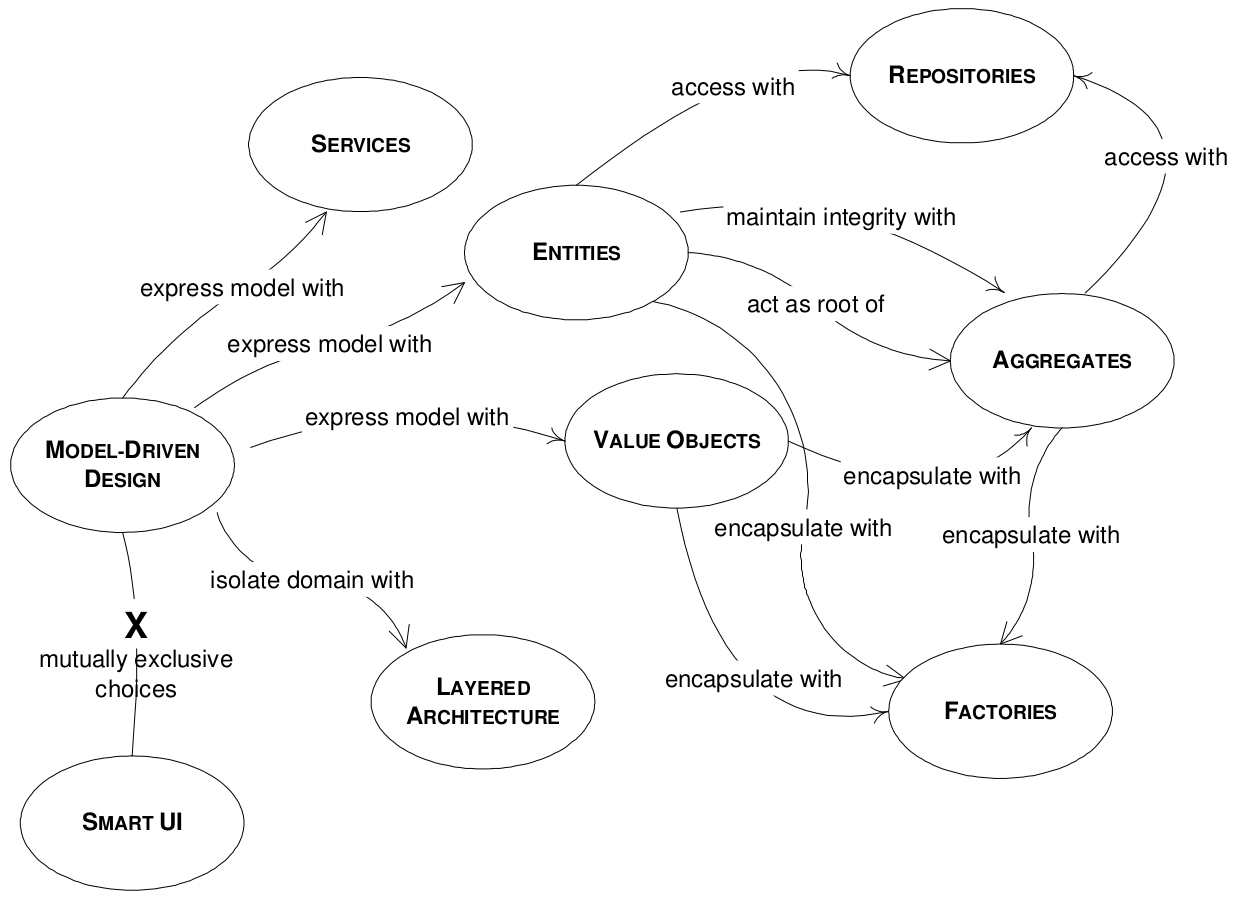
\includegraphics[width=10.5cm]{imgs/building_blocks}
	\end{center}
\end{frame}

\begin{frame}{Entidades}	
	...
\end{frame}

\begin{frame}{Objetos de Valor}	
	...
\end{frame}

\begin{frame}{Serviços}	
	...
\end{frame}

\begin{frame}{Módulos}	
	...
\end{frame}

\begin{frame}{Agregados}	
	...
\end{frame}

\begin{frame}{Fábricas}	
	...
\end{frame}

\begin{frame}{Repositórios}	
	...
\end{frame}

\section{Referências}
\begin{frame}{Referências}	
	\begin{itemize}	
		\item \href{https://github.com/johnfercher/software-literature-review}{https://github.com/johnfercher/software-literature-review}
	\end{itemize}
\end{frame}

\begin{frame}[standout]
  	Obrigado		
\end{frame}

\end{document}
